\section{Vektorrechnung}
		
	\subsection{Betrag eines Vektors}
	$$ \vert \vec{A} \vert =  \sqrt{A_x^2 + A_y^2 + A_z^2}$$
		
		
	\subsection{Gleichheit zweier Vektoren}
	Zwei Vektoren sind gleich, wenn alle Komponenten identisch sind: \\
	\\
	\begin{tabular}{ll}
	$\bullet$ & $A_x = B_x$\\
	$\bullet$ & $A_y = B_y$\\
	$\bullet$ & $A_z = B_z$\\
	\end{tabular}		
		

		
		
	\subsection{Negative eines Vektors}
	\begin{minipage}{0.6\linewidth}
	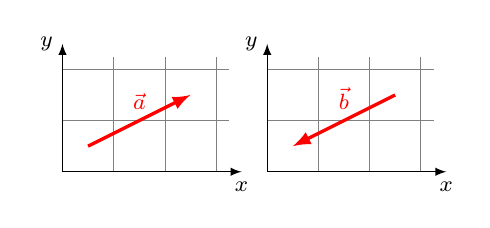
\begin{tikzpicture}
		[
		x=1cm, y=1cm, scale=0.65, font=\footnotesize, >=latex 
		%Voreinstellung für Pfeilspitzen
		]
		
		%Raster links im Hintergrund
		\draw[step=1, gray, very thin] (0,0) grid (3.25,2.25);
		
		%Länge x Achse
		\draw [-latex] (0,0) -- ++(3.5,0) node[below] {$x$};
		
		%Länge y Achse
		\draw [-latex] (0,0) -- ++(0,2.5) node[left] {$y$};	
		
		%Vektor a
		\draw[-latex, red, very thick] (0.5,0.5) -- ++(2,1) node [midway, above] {$\vec{a}$} node (a) {}; 
		
		\draw[dashed] (a.center) ++ (-3,0) node (c) {};
		
		%Raster links im Hintergrund
		\draw[step=1, gray, very thin] (4,0) grid (7.25,2.25);
		
		%Länge x Achse
		\draw [-latex] (4,0) -- ++(3.5,0) node[below] {$x$};
		
		%Länge y Achse
		\draw [-latex] (4,0) -- ++(0,2.5) node[left] {$y$};	
		
		%Vektor a
		\draw[-latex, red, very thick] (6.5,1.5) -- ++(-2,-1) node [midway, above] {$\vec{b}$} node (a) {}; 
		
	\end{tikzpicture}
	\end{minipage}
	\hfill
	\begin{minipage}{0.3\linewidth}
	$b_x = - a_x$ \\
	\\
	$b_y = - a_y$ \\
	\\
	$b_z = - a_z$ \\
	\end{minipage}	
		
		
	
	\subsection{Addition zweier Vektoren}
	
	\begin{minipage}{0.6\linewidth}
	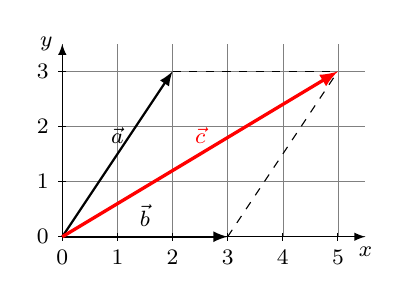
\begin{tikzpicture}
		[
		x=1cm, y=1cm, scale=0.7, font=\footnotesize, >=latex 
		%Voreinstellung für Pfeilspitzen
		]
		
		%Raster im Hintergrund
		\draw[step=1, gray, very thin] (0,0) grid (5.5,3.5);
		
		%Zahlen auf x-Achse
		\foreach \x in {0,1,2,3,4,5}
		\draw[shift={(\x,0)},color=black] (0pt,2pt) -- (0pt,-2pt) node[below]
		{\footnotesize $\x$};
		%Länge x Achse
		\draw [-latex] (0,0) -- ++(5.5,0) node[below] {$x$};
		%Länge y Achse
		\draw [-latex] (0,0) -- ++(0,3.5) node[left] {$y$};
		
		%Zahlen auf y-Achse
		%\foreach \y in {0,...,1}
		\foreach \y in {0,1,2,3}
		\draw[shift={(0,\y)},color=black] (2pt,0pt) -- (-2pt,0pt) node[left]
		{\footnotesize $\y$};		
		
		%Vektor a
		\draw[-latex, thick] (0,0) -- (2,3) node [midway, above] {$\vec{a}$} node (a) {}; 
		%Vektor b
		\draw[-latex, thick] (0,0) -- (3,0) node [midway, above] {$\vec{b}$} node (b) {}; 
		\draw[dashed] (a.center) -- ++ (3,0) node (c) {};
		\draw[dashed] (b.center) -- ++ (2,3);
		\draw[very thick, red, -latex] (0,0) -- (c.center) node [midway, above] {$\vec{c}$};
	\end{tikzpicture}
	\end{minipage}
	\hfill
	\begin{minipage}{0.3\linewidth}
	$c_x = a_x + b_x$ \\
	\\
	$c_y = a_y + b_y$ \\
	\\
	$c_z = a_z + b_z$ \\
	\end{minipage}
	
	
		
		
		
	\subsection{Subtraktion zweier Vektoren}
	
	\begin{minipage}{0.6\linewidth}
	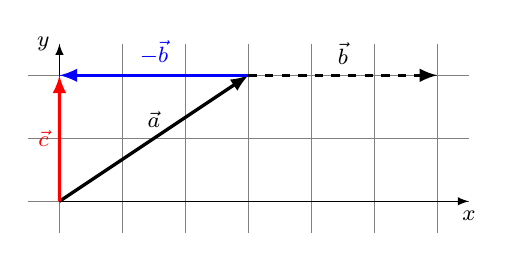
\begin{tikzpicture}
		[
		x=1cm, y=1cm, scale=0.8, font=\footnotesize, >=latex 
		%Voreinstellung für Pfeilspitzen
		]
		
		%Raster im Hintergrund
		\draw[step=1, gray, very thin] (-0.5,-0.5) grid (6.5,2.5);
		
		%Zahlen auf x-Achse
		%\foreach \x in {0,1,2,3}
		%\draw[shift={(\x,0)},color=black] (0pt,2pt) -- (0pt,-2pt) node[below]
		%{\footnotesize $\x$};
		
		%Länge x Achse
		\draw [-latex] (0,0) -- (6.5,0) node[below] {$x$};
		
		%Länge y Achse
		\draw [-latex] (0,0) -- ++(0,2.5) node[left] {$y$};	
		
		%Vektor a
		\draw[-latex, very thick] (0,0) -- (3,2) node [midway, above] {$\vec{a}$} node (a) {}; 
		
		%Vektor b
		\draw[-latex, dashed, very thick] (3,2) -- ++(3,0) node [midway, above] {$\vec{b}$} node (b) {};
		\draw[-latex, very thick, blue] (3,2) -- ++(-3,0) node [midway, above] {$-\vec{b}$} node (-b) {}; 
		\draw[dashed] (a.center) ++ (-3,0) node (c) {};
		
		%\draw[dashed] (-b.center) -- ++ (2,3);
		%\draw[dashed] (b.center) -- ++ (-1,3);
		\draw[very thick, red, -latex] (0,0) -- (c.center) node [midway, left] {$\vec{c}$};
		
		%Zahlen auf y-Achse 
		%\foreach \y in {0,...,1}
		%\foreach \y in {1,2,3}
		%\draw[shift={(0,\y)},color=black] (2pt,0pt) -- (-2pt,0pt) node[left]
		%{\footnotesize $\y$};	
	\end{tikzpicture}
	\end{minipage}
	\hfill
	\begin{minipage}{0.3\linewidth}
	$c_x = a_x - b_x$ \\
	\\
	$c_y = a_y - b_y$ \\
	\\
	$c_z = a_z - b_z$ \\
	\end{minipage}	
		
		
	\subsection{Multiplikation eines Vektros mit einem Skalar}
	\begin{minipage}{0.68\linewidth}
	$$\vec{b} = s \, \vec{a} \quad \vert \vec{B} \vert = \vert s \vert \cdot \vert \vec{a} \vert$$ \\
	\end{minipage}
	\hfill
	\begin{minipage}{0.3\linewidth}
	$b_x = s \cdot a_x$ \\
	\\
	$b_y = s \cdot a_y$ \\
	\\
	$b_z = s \cdot a_y$ \\
	\end{minipage}	
	
		
		
		
		
	\subsection{Skalarprodukt}
	$$\vec{c} = \vec{a} \bullet \vec{b} = \vert \vec{a} \vert \cdot \vert \vec{b} \, \vert  \, \cos(\varphi)$$ 
		
		
		
		
		
	\subsection{Kreuzprodukt (nur in 3D)}
	 $$\vec{a} \times \vec{b} = \begin{pmatrix} a_2 b_3 - a_3 b_2 \\ -(a_1 b_3 - a_3 b_1) \\ a_1 b_2 - a_2 b_1 \end{pmatrix}$$ 
		
				
